In this section we briefly introduce the concepts of Federated Learning, multi-party computation and Consensus Algorithms, which are used in our proposed framework.

\subsection{Federated Learning}
Federated Learning was first proposed by McMahan and the algorithm was named FedAvg\cite{mcmahan2016communicationefficient}. FedAvg requires the users to train the model on their own devices and update the parameters to the server, and the server takes the average of these parameters as the global model. FL not only helps to protect users' privacy, but also deal with the ``data in form of isolated islands'' problem for companies or institutions. Yang etc. also categorized FL into horizontal, vertical and hybrid styles based on the fact that whether the data shares the same feature space or entities\cite{yang2019federated}. 

Federated Learning can be generalized to 2 work environments:

\begin{enumerate}

    \item \textbf{Among-institutions:} In this situation FL is usually used to help companies or other institutions solving the ``data in form of isolated islands'' problem. Generally, companies and institutions are in equal status in a FL framework. Therefore, we can suppose one party can communicate with any other one privately. I.e., P2P is already enabled in this environment.

    \item \textbf{Server based:} In this case a company or institution adopt FL to train a model based on their users' data while protecting their privacy. An FL party is a common user, which means users' communication usually needs to go through the server. With an honest-but-curious server, all information will be eavesdropped by it. Therefore, problem about confidence is severe in such environment.

\end{enumerate}

Figure~\ref{fl_model} illustrates the structures of 2 environments. Executing MPC protocols and consensus algorithms is at a low price in the first environment. In the second environment, if local parameters need to be protected, we need to run some key-exchange protocols first to construct secure channels among users. Google's keyboard query suggestions\cite{yang2018applied} project was an effective application of server based federated learning. Our proposed method can work in both situations.

\begin{figure}[!ht]
    \centering
    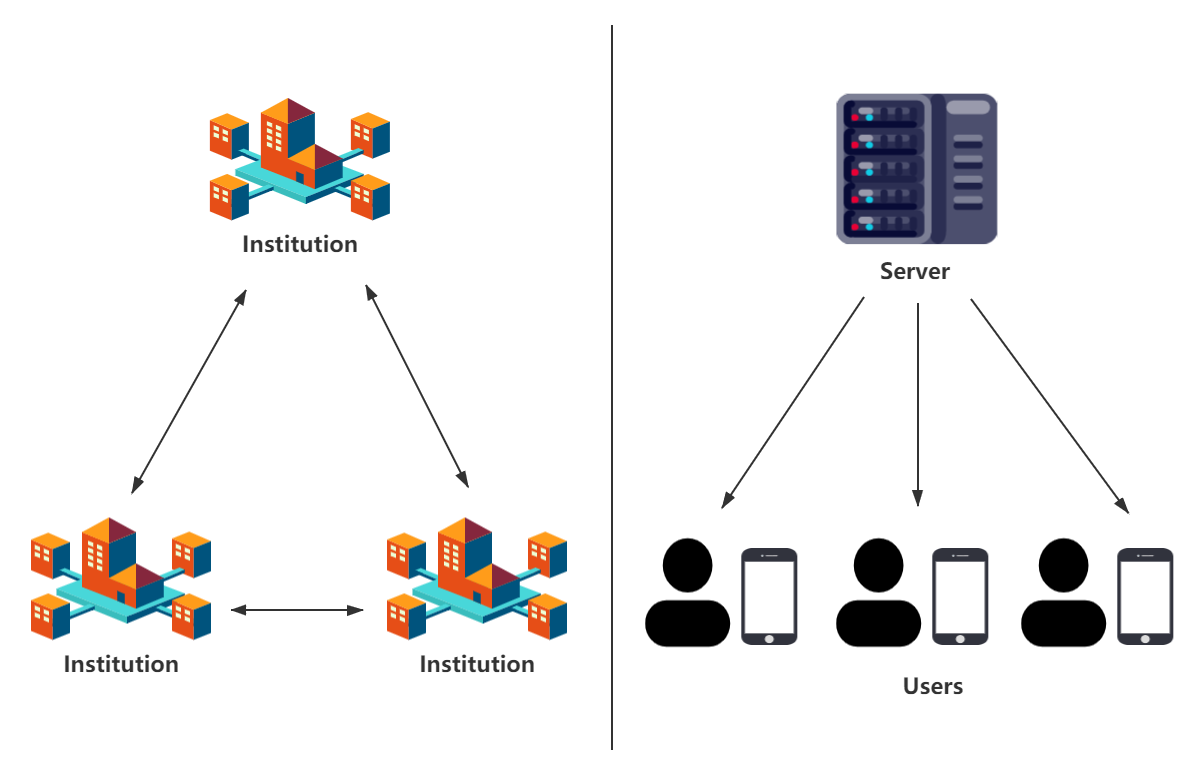
\includegraphics[width=\columnwidth]{img/fl_model.png}
    \caption{The structures of 2 work environments in Federated Learning. The left is the ``Among-institutions'' model where institutions can communicate with others directly, and the right is ``Server based'' model where parties exchange information in virtue of the server.}
    \label{fl_model}
\end{figure}


\subsection{Multi-party Computation}
Secure MPC is a branch of cryptography which enables several parties to compute a particular function without leaking their own data (inputs). It was first proposed by Yao to solve the millionaire problem\cite{Yao}. Most MPC protocols depend on two cryptography technologies: secret sharing\cite{Shamir} and oblivious transfer\cite{OT}. MPC can be implemented with garbled circuits, multi-party circuit-based protocols or hybrid methods\cite{mpc-sok}. It also benefits from fully homomorphic encryption (FHE) algorithms. Garbled circuits and FHE suffer from complicated design and poor efficiency. Therefore, secret sharing methods are more favored to solve privacy-preserving problem in FL. SPDZ\cite{SPDZ} (speedz) is a practical and secure MPC protocol introduced by Damgard etc. It supports addition and multiplication by means of the triples\cite{Triple}, which are generated by somewhat homomorphic encryption (SHE). Our method does not require multiplication and hence we does not need to generate the triples choose to use simple additive MPC.

A secret sharing scheme involves a secret $s$, a set of $n$ parties, and a collection $A$ of subsets of parties. Each party has its own share of $s$. The secret sharing scheme ensures any subset in $A$ can reconstruct $s$\cite{Secret-Sharing-survey}. By means of secret sharing we can implement secure addition among parties, which is essential in our framework.


\subsection{Consensus Algorithms}
In a distributed or multi-party system, there is always a problem about consensus. I.e., in such systems parties always need to achieve agreement on a certain value. This could be difficult without any strategy because different parties may be in different status and have multifarious matters. Consensus algorithms are adopted to solve such problems. It is widely used in blockchain and various famous areas.

Paxos was the first consensus algorithm introduced by Lamport\cite{Paxos}. It is used in a lot of famous projects such as Ceph\cite{Ceph}. Raft is a modification of Paxos which is more industrial-friendly\cite{Raft}. It contains two phases: leader election and log replication. Parties can achieve agreements based on leaders. Considering that FL model is a semi-decentralized system, our framework can utilize Raft algorithm to keep several leaders, based on which MPC protocols can be executed efficiently and robustly.
